In questo capitolo verrà descritto il programma oggetto della tesi DbN (Diagnosis by Numbers) che altro 
non è che un'estensione di \textbf{PEAR} (Probability of Exceptions and typicAlity Reasoner) \cite{PEAR}.
Inizialmente si fornirà un breve riassunto del lavoro di Soriano; successivamente cosa sia stato preso o meno.\\
Poi obiettivi posti e aggiunte ed infine il progetto completo con annesso esempio.
Come linguaggio per lo sviluppo è stato scelto \emph{Python} (in particolare la sua
versione \textit{Python3.7}) per diversi motivi, eccone alcuni:
\begin{itemize}
	\item continuità con il lavoro precedente;
	\item la presenza di nuove API (vedi \ref{sec: OwlR2} pag. \pageref{sec: OwlR2});
	\item tipicamente richiede meno codice rispetto ad altri;
	\item è uno dei linguaggi più popolari per l'elaborazione scientifica;
\end{itemize}

\section{PEAR - Sintesi}
\paragraph{Struttura}Questo tool, basato sulla logica $ \mathcal{ALC} + \mathbf{T}_{\mathbf{R}}^{\mathtt{P}} $, è strumento 
che permette di ragionare e dedurre informazioni, di definire 
precisamente chi siano gli individui tipici, atipici e quali siano
le caratteristiche peculiari di una data categoria.
Il funzionamento dell'intero strumento è riassumibile in questi passi:
\begin{enumerate}
	\item dopo aver letto le informazioni costituenti la KB, presenti in un file a parte, 
	viene creata l’ontologia;
	\item vengono combinate le probabilità delle assunzioni di tipicalità e generati tutti 
	gli scenari (possibili realtà dei fatti);
	\item di ogni scenario viene calcolata la probabilità complessiva;
	\item viene verificata o meno la consequenzialità logica del fatto $ F $ dato in input per ogni scenario;
	\item infine vengono mostrati i risultati dell'interrogazione.
\end{enumerate}
Questo è possibile anche grazie alla seguente architettura:
\begin{figure}[ht]
	\centering
	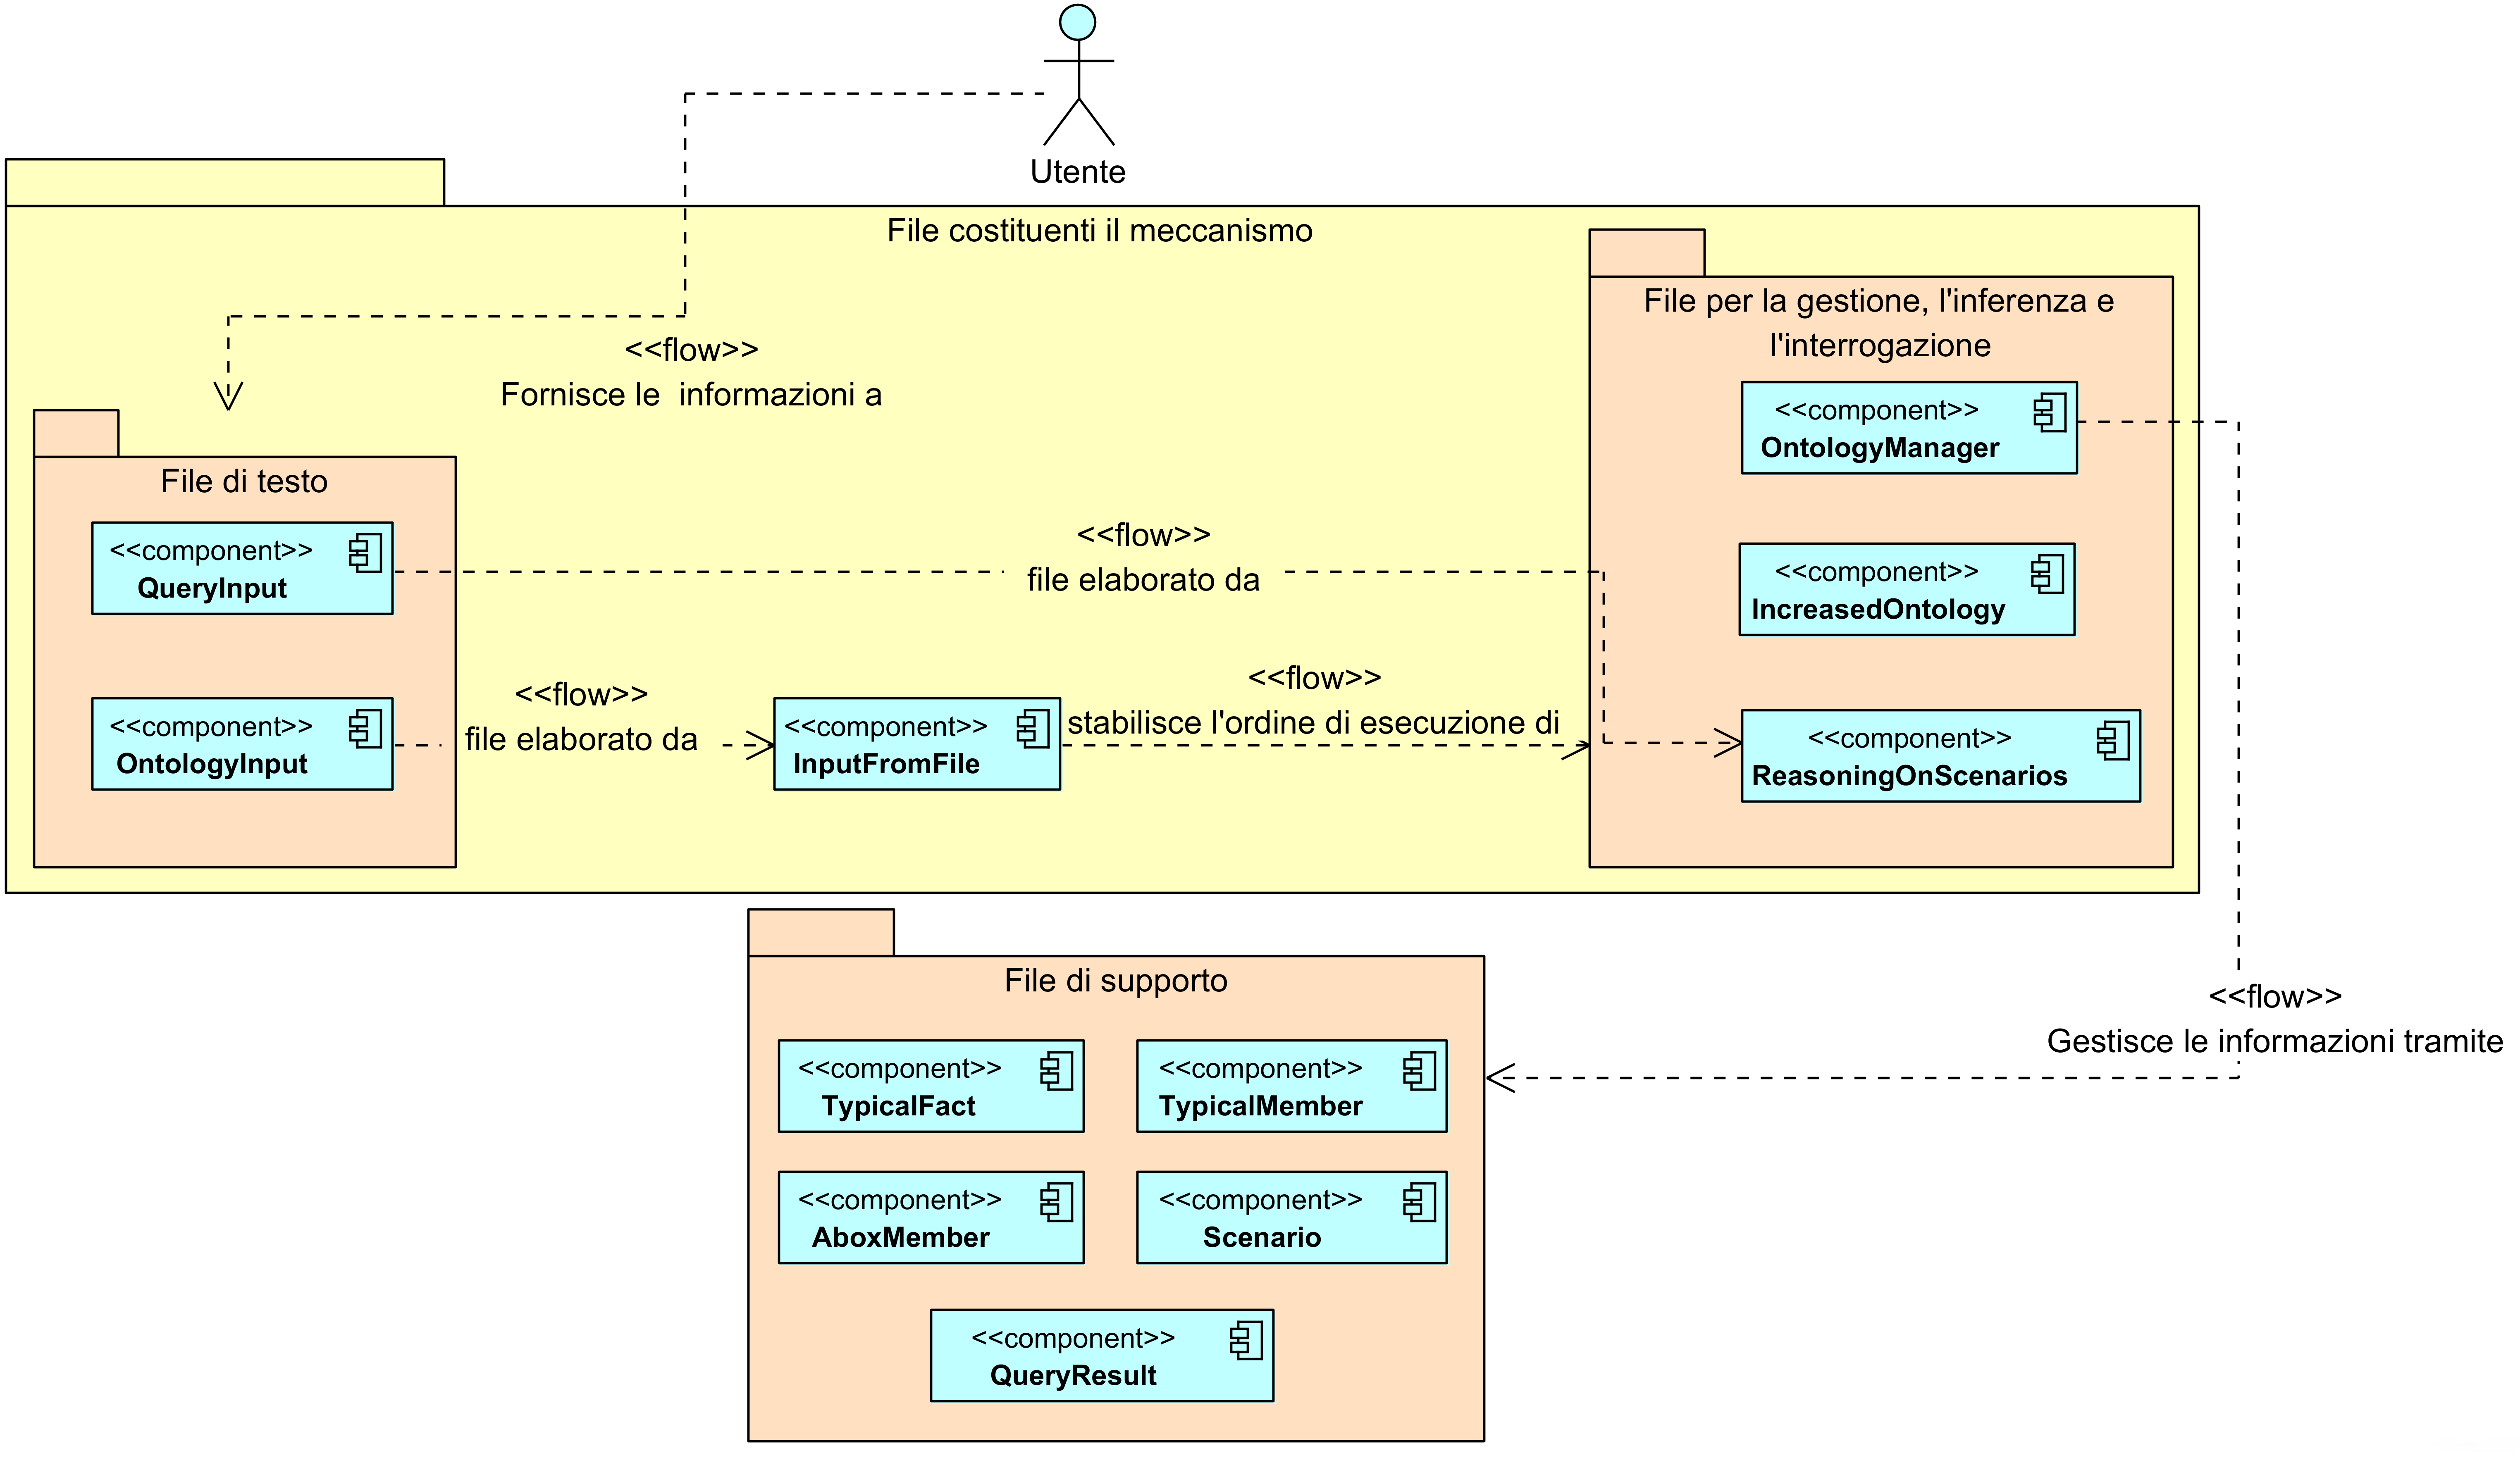
\includegraphics[width=\linewidth]{immagini/architetturaPEAR.png}
	\caption{Archittetura di Pear}
\end{figure}
dove i singoli file richiamano, spesso, i concetti teorici associati, precedentemente illustrati.
\paragraph{Limiti}
Le conclusioni così prodotte sono certamente interessanti, ma la procedura di ragionamento in se è vincolata, di volta
in volta, dalla query iniziale. \\Intuitivamente, ci si chiede se un determinato evento $ F $ sia 
conseguenza logica nella possibili diramazioni (scenari) $ B_1,B_2,....,B_n $ della base di conoscenza $ B $.
Questo procedimento non è applicabile in un contesto realistico, poiché chiederebbe all'utente di comprendere
la logica anche solo per capire come effettuare un'interrogazione significativa.
Inoltre sono presenti dei difetti tecnici, come, ad esempio, la necessità, durante la verifica di
conseguenza logica, di effettuare una copia dell'istanza del manager dell'ontologia per ogni scenario.

Alla luce di quanto detto in precedenza ecco la necessità di ottimizzazione ed espansione di PEAR in 
una naturale evoluzione: \textsl{Diagnosis by Numbers}

\section{Visione complessiva}
L'idea di questa tesi, introdotta nel capitolo 1 e ribadita più volte, finalmente inizia a prender forma.
Data un'ontologia, più o meno vasta, arricchita da espressioni di tipicalità e dai sintomi/prodromi
riguardanti un paziente, l'obiettivo è quello di generare tutte le possibili diagnosi (o spiegazioni),
controllarne la veridicità (logicamente parlando) e presentarle in forma grafica, evidenziandone la 
probabilità e il costo stimato.

Ovviamente il focus principale rimane la correttezza di esecuzione, non tanto la complessità dell'ontologia
medica o dei costi diagnostici reali. Questo non toglie che in futuro possa avere delle applicazioni concrete.

\paragraph{Struttura del progetto}
Il progetto è composto da 12 File; questi, a volte, verranno indicati con un intuitiva abbreviazione, 
così da rendere la lettura più scorrevole:
\begin{itemize}
	\item \emph{Main.py} file principale, contenente l'ordine d'esecuzione delle operazioni.
	\item Due file di testo, di input:
	\begin{itemize}
		\item \emph{OntologyInput.txt} contiene classi, relazioni tra classi, fatti tipici
			ed individui; 
		\item \emph{PatientSetOfSymptoms.txt} composto da coppie individuo-classe.
	\end{itemize}
	\item Quattro file chiave:
	\begin{itemize}
		\item \emph{OntologyManager.py} gestisce tutto ciò che riguarda l'ontologia;
		\item \emph{InputFromFile.py} si occupa della traduzione del file OntoInput tramite OntoManager;
		\item \emph{IncreasedOntology.py} calcola le probabilità di ogni membro tipico e genera tutti gli scenari;
		\item \emph{ReasoningOnScenarios.py} calcola le probabilità per ogni scenario ed effettua il ragionamento per ogni scenario arricchito con gli scenari.
	\end{itemize}
	\item Cinque file di supporto:
	\begin{itemize}
		\item \emph{AboxMember.py} corrispettivo dell'\textit{ABox};
		\item \emph{TypicalFact.py} assieme alla classe TypicalMember\\ corrispettivo dell'\textit{TBox};
		\item \emph{TypicalMember.py} assieme alla classe TypicalFact\\ corrispettivo dell'\textit{TBox};
		\item \emph{Scenario.py} rappresenta il singolo scenario;
		\item \emph{QueryResult.py} memorizza i risultati e genera il grafico associato.
	\end{itemize}
\end{itemize}
Le successive sezioni del capitolo andranno ad illustrare le funzionalità chiave dello strumento organizzate per file.
\section{Immissione dei dati}
\subsection{I documenti in ingresso}
Partiamo dall'illustrare come vengano memorizzate le informazioni relative all'ontologia dallo strumento 
e quale sia il corrispettivo del file in termini di logiche descrittive. 
\inputminted[lastline=11]{text}{codice/ExOntoInput.txt}
Il file \emph{OntologyInput.txt} è composto da 4 parti:\\
\begin{enumerate}
	\item \mintinline{text}{Classes} altro non è che un elenco di tutte le classi che si andranno ad utilizzare;
	\item \mintinline{text}{Set_as_sub_class} è una lista composta da coppie sottoclasse e classe, vedi il sottoparagrafo \ref{subSec: SintassiOWL};
	\item \mintinline{text}{Add_members_to_class} contiene gli individui e le relative classi di appartenenza; 
	\item \mintinline{text}{Set_typical_facts:} contiene l'elenco delle inclusioni di tipicalità.
\end{enumerate}

La stessa ontologia espressa in termini di \textbf{KB}$ (\mathcal{T}, \mathcal{A}) $:
\begin{itemize}
	\item $\mathcal{TB}ox$ 
		\begin{itemize}
			\item $ Bipolar \sqsubset Depressed $
			\item $ \mathbf T(ProstateCancerPatient) \sqsubseteq_{0.80} Nocturia $
			\item $ \mathbf T(Depressed) \sqsubseteq_{0.85} \neg MoodReactivity $
		\end{itemize}
	\item $\mathcal{AB}ox$ 
		\begin{itemize}
			\item $ Depressed(Greg) $
			\item $ ProstateCancerPatient(Luca) $
		\end{itemize}
\end{itemize}

In fondo al documento troviamo un nuovo elemento, i costi diagnostici; ogni malattia tipica avrà
un costo associato e, alla fine dell'elaborazione, verranno elaborati e combinati per assegnare al singolo
scenario un costo indicativo, al fine di dare un ulteriore criterio di preferenza al medico.
\inputminted[firstline=13]{text}{codice/ExOntoInput.txt}
Sotto \mintinline{text}{Set_cost_of} vi sono le coppie malattia-costo stimato (in €)

Infine il file \emph{PatientSetOfSymptoms.txt} in confronto è più basilare
\begin{minted}{text}
	Luca;Not(Bipolar) | Greg;Nocturia
\end{minted} 
Questi fatti verranno manipolati e poi aggiunti all'$ Abox$ in ogni scenario, solo se consistenti con l'ontologia di base.

\subsection{La classe dedicata alla traduzione} \label{subSec: InputFile}
Il file \emph{InputFromFile.py} contiene due metodi:
\mintinline{Python}{build_ontology} e \mintinline{Python}{read_symptoms}.
Ogni metodo si occupano del rispettivo file, rispettivamente \emph{OntologyInput.txt} e \emph{PatientSetOfSymptoms.txt}.
Infatti, dopo aver letto il contenuto del file di testo,
le stringhe vengono elaborate e successivamente data in input ai metodi della classe \mintinline{Python}{OntologyManager} quali 
\mintinline{Python}{create_class, add_sub_class_, add_member_to_class} ecc.
Come ulteriore ottimizzazione, l'esecuzione di \mintinline{Python}{read_symptoms} viene effettuata una sola volta, poiché
si è preferito salvare i dati letti in \mintinline{Python}{dict()} (coppie chiave-valore) dedicato tramite il metodo
\mintinline{Python}{store_for_reasoning}, che vedremo più in dettaglio nella prossima sezione.

Rispetto alla versione precedente il codice è stato ottimizzato e reso più leggibile anche grazie all'introduzione
di due funzioni ausiliare \mintinline{Python}{strip_not} e \mintinline{Python}{strip_typical}.
Come si intuisce dal nome lo scopo di queste 1-line-function è di rimuovere le stringhe \mintinline{Python}{"Not"}
e \mintinline{Python}{"Typical"} che son superflue e vanno diversamente gestite.

\section{L' amministrazione dell'ontologia}
Nel file \emph{OntologyManager.py}, contenente l'omonima classe, sono presenti numerosi metodi per
la creazione e la gestione dei mondi e delle ontologie. Focalizziamo la nostra attenzione sul costruttore:
\begin{minted}{Python}
def __init__(self, iri="http://www.example.org/onto.owl"):
	self.typical_facts_list = list()
	self.a_box_members_list = list()
	self.scenarios_list = list()
	self.typical_members_list = list()
	self.cost_dict = dict()
	self.symptoms_dict = dict()
	self.my_world = World()
	self.big_world = World()
	self.onto = self.my_world.get_ontology(iri)
\end{minted}
notiamo, oltre alla presenza dell'iri \ref{subSec: SintassiOWL}, l'utilizzo di una variabile, dal nome esplicativo, 
per ogni lista necessaria. La novità più importante riguarda l'utilizzo dei mondi. \textit{Owlready2 }
\ref{sec: OwlR2} può supportare numerosi mondi isolati, e questo ci aiuta, poiché siamo interessati a caricare
diverse versioni della stessa ontologia. Ecco quindi spiegate le due differenti variabili.
\mintinline{Python}{my_world} è utilizzata per contenere l'ontologia di base, mentre
\mintinline{Python}{big_world} ha lo scopo di racchiudere l'ontoBase arricchita con lo scenario selezionato.
Se non si capisce ora quale sia l'utilità di questa scelta, successivamente verrà illustrata in maniera più approfondita.

Passiamo ora ad analizzare i metodi di istanza incaricati della gestione dell'ontologia; la maggior parte sono semplici wrapper delle risorse fornite dalla libreria e non richiedono ulteriori spiegazioni. Tuttavia, 
tra questi spiccano i metodi per la gestione dei \textit{fatti tipici} e dei \textit{membri tipici}, 
operatori non conosciuti dalla nostra \textbf{API} di Python.
La soluzione migliore, già adotta in PEAR, consiste nell'eliminare l'operatore $ \mathbf T $ tramite una
particolare traduzione, vista a \ref{subSec: Traduzione T} e implementata nel metodo 
\mintinline{Python}{add_typical_fact}.
Ricordiamo, brevemente, che un paziente è atipico quando esiste \textbf{almeno un} individuo più normale di lui.
Per, invece, esprimere il concetto di membro $ m $ è un tipico $ C $ bisogna dire che $ m $ appartiene sia
alla classe $ C $ (tutti gli elementi) sia alla classe $ C1 $ (elementi tipici).
Questa idea trova la sua realizzazione nel metodo \mintinline{Python}{set_as_typical_member}.

Per ridurre i tempi di lettura e manipolazione da file si è voluto introdurre una mappa dedicata ai sintomi
con due funzioni manipolative associate, vediamole: 
\begin{minted}{Python}
def store_for_reasoning(self, member_name: str, class_id: object):
	self.symptoms_dict.update({class_id: member_name})

def add_symptoms_to_kb(self):
	for class_sy, pname, in self.symptoms_dict.items():
		class_c = self.create_class(class_sy.name)
		not_class_c = self.create_class("Not(" + class_sy.name + ")")
		class_c.equivalent_to = [Not(not_class_c)]
		self.add_member_to_class(pname, not_class_c, symp=True)
		print("Sintomo aggiunto: " + pname + ": " + class_c.name)
\end{minted}
la prima ha il compito di aggiungere valori al "dizionario" le coppie:\\ \mintinline{Python}{nome-paziente: classe-sintomo}.\\
La seconda, invece, per ogni coppia presente nella struttura, crea le classi appropriate e poi 
aggiunge un membro all'\textit{ABox} all'ontologia corrente tramite la funzione \mintinline{Python}{add_member_to_class}.

È altrettanto importante focalizzarci sulla gestione dei mondi, effettuata dai metodi:
\begin{minted}{Python}
	def save_base_world(self):
	 self.onto.save("ontoBase.owl", format="ntriples")
	
	def create_new_world(self):
	 self.onto.destroy()
	 self.big_world = World()
	 self.onto = self.big_world.get_ontology(
	 "file://" + PATH_TO_ONTO + "//ontoBase.owl").load() 
\end{minted}
il primo possiede l'incarico di esportare l'ontologia, creata nell'omonimo mondo nel punto 
\ref{subSec: InputFile}
Il secondo assume la funzione di distruggere l'ontologia contenuta nella variabile \textit{onto}, 
di creare un nuovo mondo e di caricare l'ontologia salvata precedentemente sul file.
Vedremo meglio più avanti quale sia stata la strategia dietro lo sviluppo di questi metodi.\\
Analogamente a questo concetto citiamo la seguente funzione:
\begin{minted}{Python}
def consistency(self, condition: bool = False):
	try:
	with self.onto:
		if condition:
			sync_reasoner(self.my_world)
			classi_incosistenti = list(
 				self.my_world.inconsistent_classes())
			if not len(classi_incosistenti) == 0:
 				return classi_incosistenti
		else:
			sync_reasoner(self.big_world)
   		return "The ontology is consistent"
	except OwlReadyInconsistentOntologyError:
 		return "The ontology is inconsistent"
\end{minted}
I ragionatore \emph{Hermit} è in grado di controllare la consistenza di un ontologia e dedurre nuovi fatti,
riclassificando individui e classi in base alle loro relazioni. In caso di inconsistenza viene lanciata
l'eccezione appropriata. È possibile avere classi inconsistenti senza rendere l'intera ontologia
inconsistente ,a patto che queste non abbiano individui. In nostro aiuto il reasoner inferisce tali classi
come equivalenti to \textbf{Nothing} (elemento primitivo di OWL) ed è quindi possibile interrompere 
l'esecuzione del tool prima che l'intera ontologia sia inconsistente!
Vediamo un esempio. Se avessi una \textbf{KB}:
\begin{multicols}{2}
	\textit{TBox}
	\begin{itemize}
		\item $ \neg A \sqsubseteq B $
		\item $ B \sqsubseteq A $
		\item $ \mathbf{T}(C) \sqsubseteq_{0.80} D $
	\end{itemize}
	\columnbreak
	\textit{ABox}
	\begin{itemize}
		\item $ D(Giovanni) $
	\end{itemize}
\end{multicols}
La classe $ \neg A $, nonostante non abbia elementi, è inconsistente poiché in contraddizione con
l'assioma $ B \sqsubseteq A $. Questo chiude la trattazione del manager.

\section{La creazione dei membri tipici e degli scenari}
Il file \emph{IncreasedOntology.py} è un modulo che fornisce i metodi necessari per la
generazione di tutti i membri tipici e gli scenari possibili e per il calcolo delle relative probabilità.
I metodi incaricati del valutazione delle "percentuali" sono:
\begin{minted}{Python}
def compute_probability_for_typical_members(onto_manager):
	facts_list = onto_manager.typical_facts_list
	abox_members_list = onto_manager.a_box_members_list
	facts_list.sort(key=lambda x: x.t_class_identifier.name)
	abox_members_list.sort(key=lambda x: x.class_identifier.name)
	......
    __set_probability( prob_to_assign_to_typical_member, onto_manager,
    	facts_list[i].t_class_identifier,
    	facts_list[i].class_identifier)
	....
	
def __set_probability(prob_to_assign, onto_mng, t_class_id, class_id):
	for aboxMember in onto_mng.a_box_members_list:
		if aboxMember.isSymptom is True and
		 aboxMember.class_identifier.name == class_id.name:
			onto_mng.typical_members_list.
			append(TypicalMember(
				t_class_id,
				aboxMember.member_name,
				prob_to_assign
			))
\end{minted}
Il primo processo è il più complicato e si avvale del secondo come supporto.
In sintesi per computare la probabilità da associare ad ogni membro tipico si 
vanno a moltiplicare tra loro le probabilità di ogni inclusione di tipicalità avente la
medesima classe argomento dell’operatore $ \mathbf{T} $
(ovvero \mintinline{Python}{t_class_identifier}) e, a quel punto, il metodo
di supporto,viene invocato per creare il membro tipico.

Ricordiamo che $ m $ è tipico se è nella forma $ p:\mathbf{T}(C)(m) $.
Tale funzione, quindi, scansionando tutti i membri dell'\textit{ABox}, cerca quello che è un sintomo
e ha come classe di appartenenza $ C $. Una volta trovato, passa alla creazione Membro tipico, con la 
probabilità calcolata precedentemente.

La seconda parte della classe ha la responsabilità degli scenari, realtà possibili dei fatti.
Il numero totale cambia al variare dei \mintinline{Python}{TypicalMember} e del numero di Sintomi,
in particolare, con $ n $ membri tipici è $ 2^{n} $. Considerando, ad esempio, $ mt1 $ e $ mt2 $
l'insieme risultante sarà la combinazione:
\[ \{\{\emptyset\},\{mt1\},\{mt2\},\{mt1,mt2\}\} \]
dove $ \emptyset $ rappresenta lo scenario vuoto, in cui non si fa alcuna assunzione, $ \{mt1\} $
in cui si assume solo $ mt1 $, $ \{mt2\} $ in cui si assume solo $ mt2 $ e infine l'ultimo 
dove si assumono entrambi.

Per quanto riguarda la probabilità da associare ad ogni scenario, essa è data dal 
prodotto di $ k $ fattori, con $ k $ pari al numero di membri tipici generati (nell’esempio
precedente avendo due \mintinline{Python}{TypicalMember}, la probabilità di ognuno dei 
quattro scenari è data dal prodotto di $ k = 2 $ fattori) dove ogni fattore è una probabilità 
che coincide con la $ p $ appartenente al membro tipico  se assunto, 
altrimenti vale $ 1 - p $ se questo, nello scenario, non viene assunto.\\
Riprendendo l’esempio precedente, supponendo che $ mt1 $ abbia come probabilità il valore $ p1 $ 
e che $ mt2 $ abbia il valore $ p2 $, la probabilità dello scenario vuoto vale $ ( 1 - p1) \ ( 1 - p2)$,
quella dello scenario in cui si assume solo $ mt1 $ vale $ p1 \times ( 1 - p2) $, 
quella in cui si assume solo $ mt2 $ vale $ ( 1 - p1) \times p2 $ ed infine l’ultimo scenario $ p1 \times p2 $.

I metodi che si occupano di questa traduzione sono 4, 1 principale e 3 di supporto "privati":
\begin{minted}{Python}
def set_probability_for_each_scenario(ontology_manager):
def __generate_scenario(ontology_manager):
def __difference(scenario, typical_members_list):
def __get_typical_member(key, ontology_manager):
\end{minted}
Per prima cosa il metodo \mintinline{Python}{set_probability_for_each_scenario} 
genera tutti gli scenari tramite il metodo \mintinline{Python}{__generate_scenario} (determinando
l’insieme delle parti), successivamente gli scenari vengono così processati:
viene moltiplicata la probabilità dei membri tipici assunti e non assunti 
(grazie a \mintinline{Python}{__difference}) in modo da calcolare la probabilità per ogni scenario.
Questo verrà memorizzato nell'oggetto dedicato \mintinline{Python}{Scenario}
 ovviamente gestito dall'\mintinline{Python}{OntologyManager}.

In particolare il metodo \mintinline{Python}{__difference} effettua una 
differenza insiemistica tra i due insiemi: membri tipici: assunti e generati. 
\mintinline{Python}{__get_typical_member}, invece, calcola la probabilità del membro tipico non assunto
nello scenario corrente grazie alla presenza delle chiavi identificative \mintinline{Python}{key}:
cerca all'interno dell'\mintinline{Python}{ontology_manager} l’oggetto \mintinline{Python}{TypicalMember} corrispondente a quella chiave.

Abbiamo deciso di ignorare lo scenario $ \emptyset $ poiché è il più banale, già scartato in altri contesti.
Infatti è corretto logicamente generare tale scenario ma, verificato o meno se sia conseguenza logica della KB,
non ha molto senso dare una diagnosi del tipo: con una probabilità X non ha niente.

\section{L'inferenza}
Il file \emph{ReasoningOnScenarios.py} si occupa di verificare se i sintomi in input
seguano logicamente dalla base di conoscenza, arricchita con l'aggiunta di un determinato scenario.
Questo per ogni oggetto \mintinline{Python}{Scenario} presente.
Per verificare l'\textit{implicazione logica}, in simbolo $  A \models B $, bisogna verificare che
in tutti i modelli in cui $ A $ è $ True $, anche $ B $ è vera. Nel nostro caso dobbiamo provare
che $ KB \cup S \models V $ dove $ S $ è un determinato scenario e $ V $ è un set di formule che
rappresenta i sintomi del paziente. Possiamo dimostrare ciò grazie 
alla dimostrazione per \textbf{refutazione}, che permette di
rispondere $ True $ se si dimostra l'equivalenza $ (KB \cup S \wedge\neg V) \equiv False $.
DbN utilizzerà proprio questa strategia, vediamo come.
\begin{minted}{Python}
def __translate_scenario(scenario, ontology_manager):
	for tm in scenario.list_of_typical_members:
		ontology_manager.set_as_typical_member(
			tm.member_name, tm.t_class_identifier, 
			ontology_manager.
			onto[tm.t_class_identifier.name + "1"])
def is_logical_consequence(ontology_manager, 
	lower_probability_bound=0, higher_probability_bound=1):
\end{minted}
Il metodo, di supporto, \mintinline{Python}{translate_scenarios} ha il compito di tradurre 
ogni membro tipico presente all’interno dello scenario.
Il metodo \mintinline{Python}{is_logical_consequence} gestisce l'intera fase di verifica, 
opzionalmente esaminando solo gli scenari in un determinato intervallo di probabilità, tramite
gli argomenti facoltativi lower and higher \mintinline{Python}{_bound}.
I risultati verranno salvati all'interno di \mintinline{Python}{query_result = QueryResult()}.
Una volta selezionati gli scenari, questi vengono esaminati uno per volta nel seguente modo:
\begin{enumerate}
	\item viene creato un nuovo \mintinline{Python}{mondo}, un'universo isolato, in cui si carica
	 	l'ontologia di base creata in precedenza;
	\item a questa vengono aggiunti i sintomi \textbf{negati} e lo scenario corrente, tramite i metodi
	 \mintinline{Python}{add_symptoms_to_kb()} e \mintinline{Python}{__translate_scenario()};
	\item quindi si verifica la consistenza dell'ontologia:
	\begin{itemize}
		\item se è consistente, cioè $ \equiv True $, allora $ KB \cup S \not\models V $ 
			e quindi lo scenario viene ignorato e il ciclo riparte \textbf{loop}.
	\end{itemize}
	\item In caso contrario, si salva l'oggetto \mintinline{Python}{Scenario} 
		all'interno di \mintinline{Python}{query_result};
	\item e si accumula la probabilità dello scenario, appena verificato, \\
		nella var \mintinline{Python}{total_probability}, riparte il \textbf{loop}; 		
\end{enumerate}
Alla fine del ciclo si salva la probabilità totale così all'interno della variabile\\ \mintinline{Python}{query_result}. L' esecuzione quindi termina.

\section{Analisi del risultato}
Alla luce di quanto detto prima, vediamo ora la struttura del file \emph{QueryResult.py} e, 
in particolare, delle sue operazioni.
\begin{minted}{Python}
def show_query_result(self):
	.....
def create_and_show_plot(self, patient_symptoms: str, disease_cost: dict):
	# Crea una figura con un secondo asse y
	self.fig = make_subplots(specs=[[{"secondary_y": True}]])
	# Crea l'istogramma, come asse y la probabilità degli scenari
	trace1 = go.Bar(...)
	# Aggiunge quest'ultimo alla figura
	self.fig.add_trace(trace1)
	# Crea il grafico a dispersione, come asse y il costo degli scenari €
	trace2 = go.Scatter(...)
	# Viene unito alla figura, specificando della presenza del diverso asse y
	self.fig.add_trace(trace2, secondary_y=True)	
	self.fig.show()
\end{minted}
La prima funzione ha il compito di stampare, sullo standar output, gli scenari possibili.
Più interessante è \mintinline{Python}{create_and_show_plot}, questa, grazie all'utilizzo di
Plotly (vedi \ref{sec: Plotly} a pag. \pageref{sec: Plotly}), permette la realizzazione di un grafico
interattivo, contente tutte le informazioni significative e facilmente esplorabile.
L'idea è stata quella di utilizzare due grafici distinti per rappresentare la probabilità e 
i costi dei singoli scenari, vedi la Figura \ref{fig:duePlotDistinti}.
Successivamente si è pensato di unire i due grafici, poiché accomunati dagli stessi valori sull'asse delle x,
semplicemente il numero dello scenario generato; il risultato è stato, all'incirca, questo è mostrato
nella Figura \ref{fig:duePlotUniti}.
Per migliorare il risultato finale sono stati aggiunti ulteriori metadati, così da rendere il grafico
il più auto-esplicativo possibile. Vale la pena menzionare la possibilità di esportare e salvare i risultati
in due formati distinti. Html per una visione dinamica, mentre pdf per una statica.
\begin{minted}{Python}
def save_query_result(self,name=None):
	if name is not None:
		# self.fig.write_html(name + ".html")
		self.fig.write_image(name + ".pdf")
\end{minted}
\begin{figure}[h]
	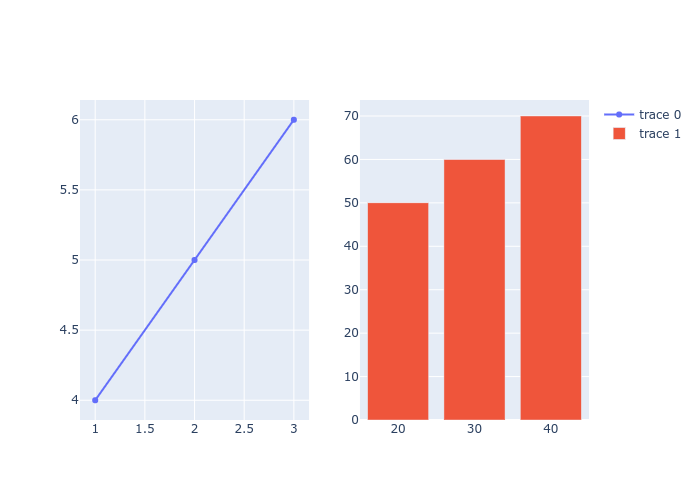
\includegraphics[width=\linewidth]{plot/plotly_two_graph.png}
	\caption{Grafico a dispersione e Istogramma separati}
	\centering
	\label{fig:duePlotDistinti}
\end{figure}
\begin{figure}[h]
	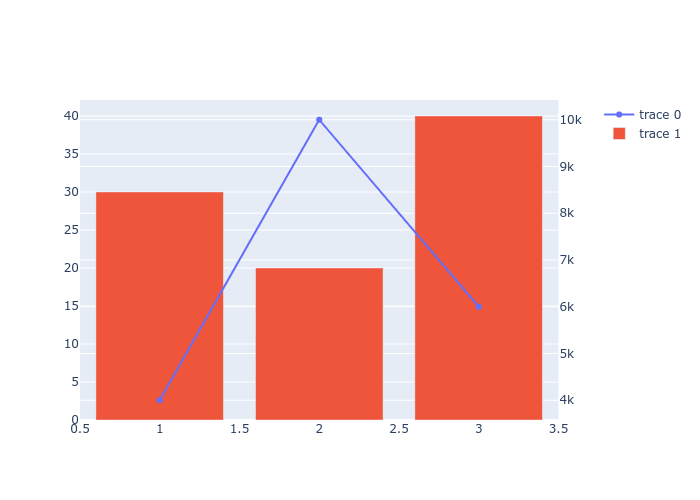
\includegraphics[width=\linewidth]{plot/plot_mixed.png}
	\caption{Grafico a dispersione e Istogramma uniti}
	\centering
	\label{fig:duePlotUniti}
\end{figure}
\clearpage

\section{Il file principale \emph{Main.py}}
Composto  dal omonimo \mintinline{Python}{__name__ == '__main__'} e dalla nuova funzione di 
supporto \mintinline{Python}{entailed_knowledge()}.
\begin{minted}{Python}
def entailed_knowledge():
	patient_sym = read_symptoms(ontology_manager, result=True)
	result = ontology_manager.consistency(condition=True)
	if not result == "The ontology is consistent":
		# Ontologia inconsistente o classi inconsitenti
		print(result)
		ontology_manager.show_classes_iri_my()
		ontology_manager.show_members_in_classes_my()
		# Termina
		sys.exit(5)
	return patient_sym
\end{minted}
In quest'ultima effettua la lettura dei sintomi (vedi \ref{subSec: InputFile}) e salvato il
valore di ritorno si verifica la consistenza della \textbf{KB}. In caso negativo si effettuano delle stampe esplicative e si termina l'esecuzione; altrimenti si ritorna i sintomi, sotto forma di stringa.
                
Il \mintinline{Python}{'__main__'} altro non è che la corretta sequenza di chiamate che 
permette al tool di funzionare: 
\begin{minted}{Python}
if __name__ == '__main__':
	ontology_manager = OntologyManager()
	build_ontology(ontology_manager)
	sym: str = entailed_knowledge()
	IncreasedOntology.compute_probability_for_typical_members(ontology_manager)
	IncreasedOntology.set_probability_for_each_scenario(ontology_manager)
	ontology_manager.show_scenarios()
	query_result = is_logical_consequence(ontology_manager)
	query_result.show_query_result()
	query_result.create_and_show_plot(sym, ontology_manager.cost_dict)
\end{minted}
in primis viene istanziata la classe \mintinline{Python}{OntologyManager}, 
dopodichè viene invocato il metodo \mintinline{Python}{build_ontology} tramite cui viene costruita l'ontologia ed ecco quindi la chiamata all'attività di supporto.
Calcolata le probabilità necessarie per i membri tipici e per gli scenari generati, si passa
alla fase di inferenza e successivamente a quella di analisi dei risultati e generazione dei
grafici. Questo conclude la simulazione.

Abbiamo trattato lo strumento nel modo più completo possibile, cercando, però, di evitare
dettagli o piccolezze trascurabili, focalizzando l'attenzione il più possibile sugli
elementi importanti e peculiari.

                                                            
\begin{comment}

\begin{figure}
\centering
\includegraphics[width=\linewidth]{plot/DepressionEx2.pdf}
\end{figure}
\end{comment}


